% Provenance (never printed): old seconde/premiere S material on the
% atmosphere (water vapour, saturation, cloud formation, the vertical motion
% of air) and enseignement scientifique premiere (water cycle); see
% sources/book2/PROVENANCE.md. Every saturation value, lapse rate,
% condensation level and the lee-wind example are computed in
% figdata/grade-10/clouds.py from the IAPWS saturation curves; the soundings
% are invented examples, said so in the text.
\chapter{Pourquoi les nuages se forment}\label{ch:g10:why-clouds-form}

Sur une terrasse en été, un verre d'eau glacée est posé sur une table. En
moins d'une minute, sa paroi extérieure se couvre de gouttelettes, et un
cercle d'eau s'étale à son pied. L'eau n'a pas traversé le verre~: elle
vient de l'air, refroidi là où il touchait le verre froid. Quelques heures
plus tard, à des kilomètres au-dessus de la plaine, la même chose se produit
en grand~: des bulles d'air chaud montent, se refroidissent, et à une
certaine altitude l'eau qu'elles transportent apparaît sous forme de ces
amas de nuages blancs à base plate qu'on appelle cumulus. Ce chapitre
explique quelle quantité de vapeur d'eau l'air peut contenir, pourquoi l'air
qui monte se refroidit, à quelle altitude se forment les nuages, pourquoi
certains jours ils restent plats et d'autres s'élèvent en orages, et
comment de minuscules gouttelettes de nuage deviennent pluie et neige.

\begin{omfigure}
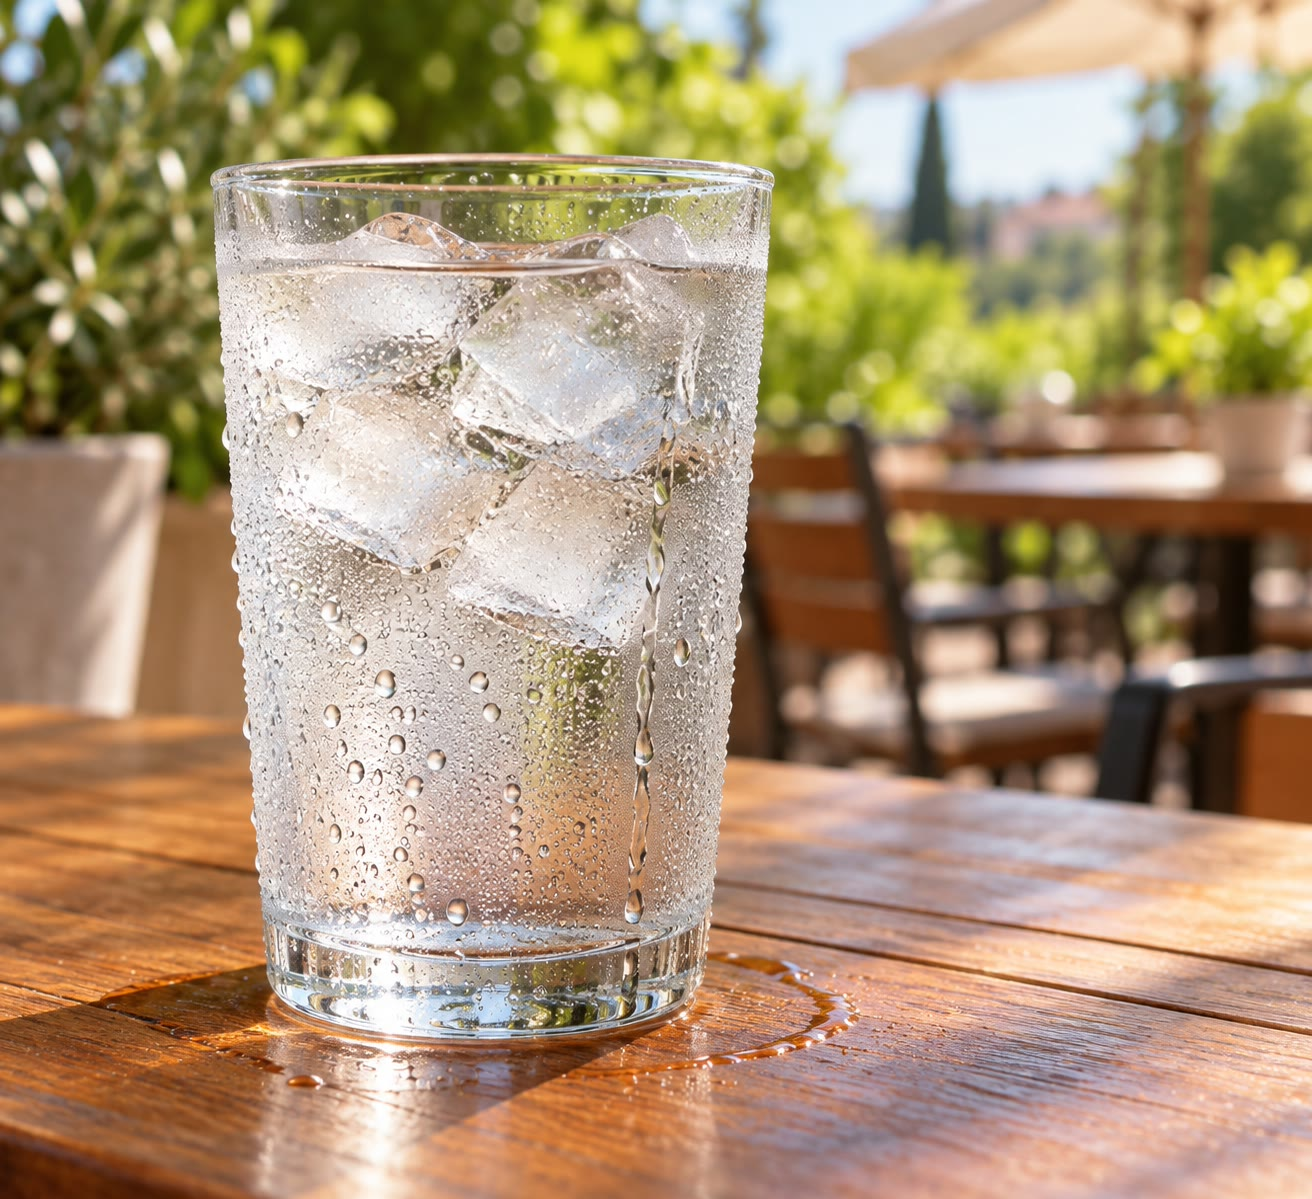
\includegraphics[width=0.5\linewidth]{images/book2/ai/g10-cold-glass.jpg}

{\small Un verre d'eau glacée sur une terrasse en été~: des gouttes se
forment sur sa paroi extérieure, là où l'air qui touche le verre se
refroidit.}
\end{omfigure}

\begin{recall}
Les nuages sont faits de minuscules gouttelettes d'eau ou de cristaux de
glace~; on les classe en familles d'après leur forme et leur altitude, et
ils donnent la pluie, la neige et la grêle, que l'on mesure avec un
pluviomètre (livre~1, année~4). Dans la couche la plus basse de
l'atmosphère, la température de l'air diminue avec l'altitude, en moyenne
d'environ \qty{6.5}{\degreeCelsius} par kilomètre~; c'est le gradient
thermique vertical, et les fronts séparent des masses d'air de températures
différentes (livre~1, année~8). La pression diminue avec l'altitude (les
livres de physique). L'eau s'évapore et se condense, et l'évaporation
absorbe une \omterm{def:g10:earth-energy-budget:latent-heat}{chaleur latente} que la condensation restitue (les livres de
physique et le \cref{ch:g10:earth-energy-budget}).
\end{recall}
% ledger: nasa:grc-atmosphere

\section{La vapeur d'eau et la saturation}

L'air contient toujours de la vapeur d'eau, un gaz invisible. La quantité
qu'il peut en contenir dépend avant tout de sa température.

\begin{definition}[Saturation~; humidité relative]\label{def:g10:why-clouds-form:humidity}
L'air est \emph{saturé}\index{saturation} lorsqu'il contient la plus grande
masse de vapeur d'eau qu'il peut contenir à sa température, sa \emph{teneur
à saturation}~; toute vapeur supplémentaire se condense en gouttelettes.
L'\emph{humidité relative}\index{humidite relative@humidité relative} de
l'air est sa teneur en vapeur d'eau divisée par sa teneur à saturation à la
même température et à la même pression, exprimée en pourcentage.
\end{definition}

La teneur en eau de l'air se mesure ici en grammes de vapeur par kilogramme
d'air sec (\unit{g/kg})~: une parcelle d'air qui monte ou descend sans
gagner ni perdre d'eau garde la même teneur, même en se dilatant.

\begin{omfigure}
\begin{tikzpicture}
\begin{axis}[omrecord, width=0.88\linewidth, height=6.2cm, xmin=-10, xmax=40,
  ymin=0, ymax=50, xlabel={température (\unit{\degreeCelsius})},
  ylabel={teneur à saturation (\unit{g/kg})}, xtick={-10,0,...,40},
  tick label style={font=\small}, label style={font=\small}]
\addplot[omDef!85!black, thick] table[x=T_C, y=ws_gkg] {figdata/out/grade-10-clouds-sat.dat};
\addplot[only marks, mark=*, mark size=1.8pt, omThm!85!black] coordinates {(28,11.37)};
\addplot[only marks, mark=o, mark size=1.8pt, omThm!85!black] coordinates {(16,11.37)};
\draw[->, omThm!85!black, thick] (axis cs:27.2,11.37) -- (axis cs:16.9,11.37);
\node[anchor=north, font=\footnotesize, omThm!85!black] at (axis cs:28,10.6) {air à \qty{28}{\degreeCelsius}};
\node[anchor=south east, font=\footnotesize, omThm!85!black] at (axis cs:15.5,12.2) {point de rosée};
\node[anchor=south east, font=\footnotesize, omDef!85!black, align=right] at (axis cs:31,34) {au-dessus de la courbe~:\\la vapeur se condense};
\node[anchor=south west, font=\footnotesize, omDef!85!black] at (axis cs:31,2.5) {non saturé};
\node[anchor=north west, font=\footnotesize, omDef!85!black] at (axis cs:34,31.5) {saturation};
\end{axis}
\end{tikzpicture}

{\small La plus grande masse de vapeur d'eau qu'un kilogramme d'air peut
contenir, en fonction de la température, à la pression du niveau de la mer
(au-dessus de l'eau liquide~; calculée d'après la norme internationale sur
l'eau). De l'air à \qty{28}{\degreeCelsius} qui contient \qty{11.4}{g/kg}
(point plein) est loin de la \omterm{def:g10:why-clouds-form:humidity}{saturation}~; refroidi sans perdre d'eau, il
devient \omterm{def:g10:why-clouds-form:humidity}{saturé} à \qty{16}{\degreeCelsius} (cercle).}
\end{omfigure}
% ledger: iapws:vapour-pressure, ciaaw:abridged-2024, earth:Mmol, const:R (computed in figdata/grade-10/clouds.py)

La courbe monte fortement~: \qty{3.8}{g/kg} à \qty{0}{\degreeCelsius},
\qty{14.7}{g/kg} à \qty{20}{\degreeCelsius}, \qty{27.2}{g/kg} à
\qty{30}{\degreeCelsius}. Chaque réchauffement de \qty{10}{\degreeCelsius}
double presque l'eau que l'air peut contenir. C'est pourquoi l'air tropical
peut apporter des pluies torrentielles, et pourquoi l'air d'un hiver
polaire, même \omterm{def:g10:why-clouds-form:humidity}{saturé}, ne contient presque rien.

\begin{definition}[Point de rosée]\label{def:g10:why-clouds-form:dew-point}
Le \emph{point de rosée}\index{point de rosee@point de rosée} de l'air est
la température à laquelle il faut le refroidir, en conservant sa teneur en
eau et sa pression, pour qu'il devienne \omterm{def:g10:why-clouds-form:humidity}{saturé}.
\end{definition}

\begin{method}[Humidité relative et point de rosée à partir d'un tableau]\label{met:g10:why-clouds-form:table}
\begin{enumerate}
  \item Lire dans le tableau la teneur à \omterm{def:g10:why-clouds-form:humidity}{saturation} à la température de
        l'air.
  \item \omterm{def:g10:why-clouds-form:humidity}{Humidité relative}~: diviser la teneur en eau de l'air par cette
        valeur.
  \item \omterm{def:g10:why-clouds-form:dew-point}{Point de rosée}~: chercher dans le tableau la température dont la
        teneur à \omterm{def:g10:why-clouds-form:humidity}{saturation} est égale à la teneur en eau de l'air.
\end{enumerate}
\end{method}

\begin{example}[Un matin d'été]\label{ex:g10:why-clouds-form:morning}
% ledger: iapws:vapour-pressure (values computed in figdata/grade-10/clouds.py)
À \qty{20}{\degreeCelsius}, l'air contient \qty{11.4}{g/kg}. La teneur à
\omterm{def:g10:why-clouds-form:humidity}{saturation} à \qty{20}{\degreeCelsius} est de \qty{14.7}{g/kg}, donc
l'\omterm{def:g10:why-clouds-form:humidity}{humidité relative} vaut $11.4/14.7 \approx \qty{78}{\percent}$. La teneur à
\omterm{def:g10:why-clouds-form:humidity}{saturation} vaut \qty{11.4}{g/kg} à \qty{16}{\degreeCelsius}~: c'est le
\omterm{def:g10:why-clouds-form:dew-point}{point de rosée}. L'après-midi, le même air réchauffé à
\qty{28}{\degreeCelsius} (teneur à \omterm{def:g10:why-clouds-form:humidity}{saturation} \qty{24.1}{g/kg}) n'a plus
qu'une \omterm{def:g10:why-clouds-form:humidity}{humidité relative} de \qty{47}{\percent} --- avec exactement la même
eau.
\end{example}

Le verre de l'introduction est plus froid que le \omterm{def:g10:why-clouds-form:dew-point}{point de rosée} de l'air
qui l'entoure~: l'air à son contact est refroidi sous son \omterm{def:g10:why-clouds-form:dew-point}{point de rosée} et
dépose de l'eau sur le verre. Par une nuit claire, l'herbe et les toits des
voitures perdent de la chaleur en rayonnant de l'infrarouge vers le ciel et
deviennent plus froids que l'air~: la rosée s'y forme, ou le givre en
dessous de \qty{0}{\degreeCelsius}. Quand toute une couche d'air proche du
sol se refroidit jusqu'à son \omterm{def:g10:why-clouds-form:dew-point}{point de rosée}, des gouttelettes se forment
dans l'air lui-même~: c'est le brouillard.

\begin{omfigure}
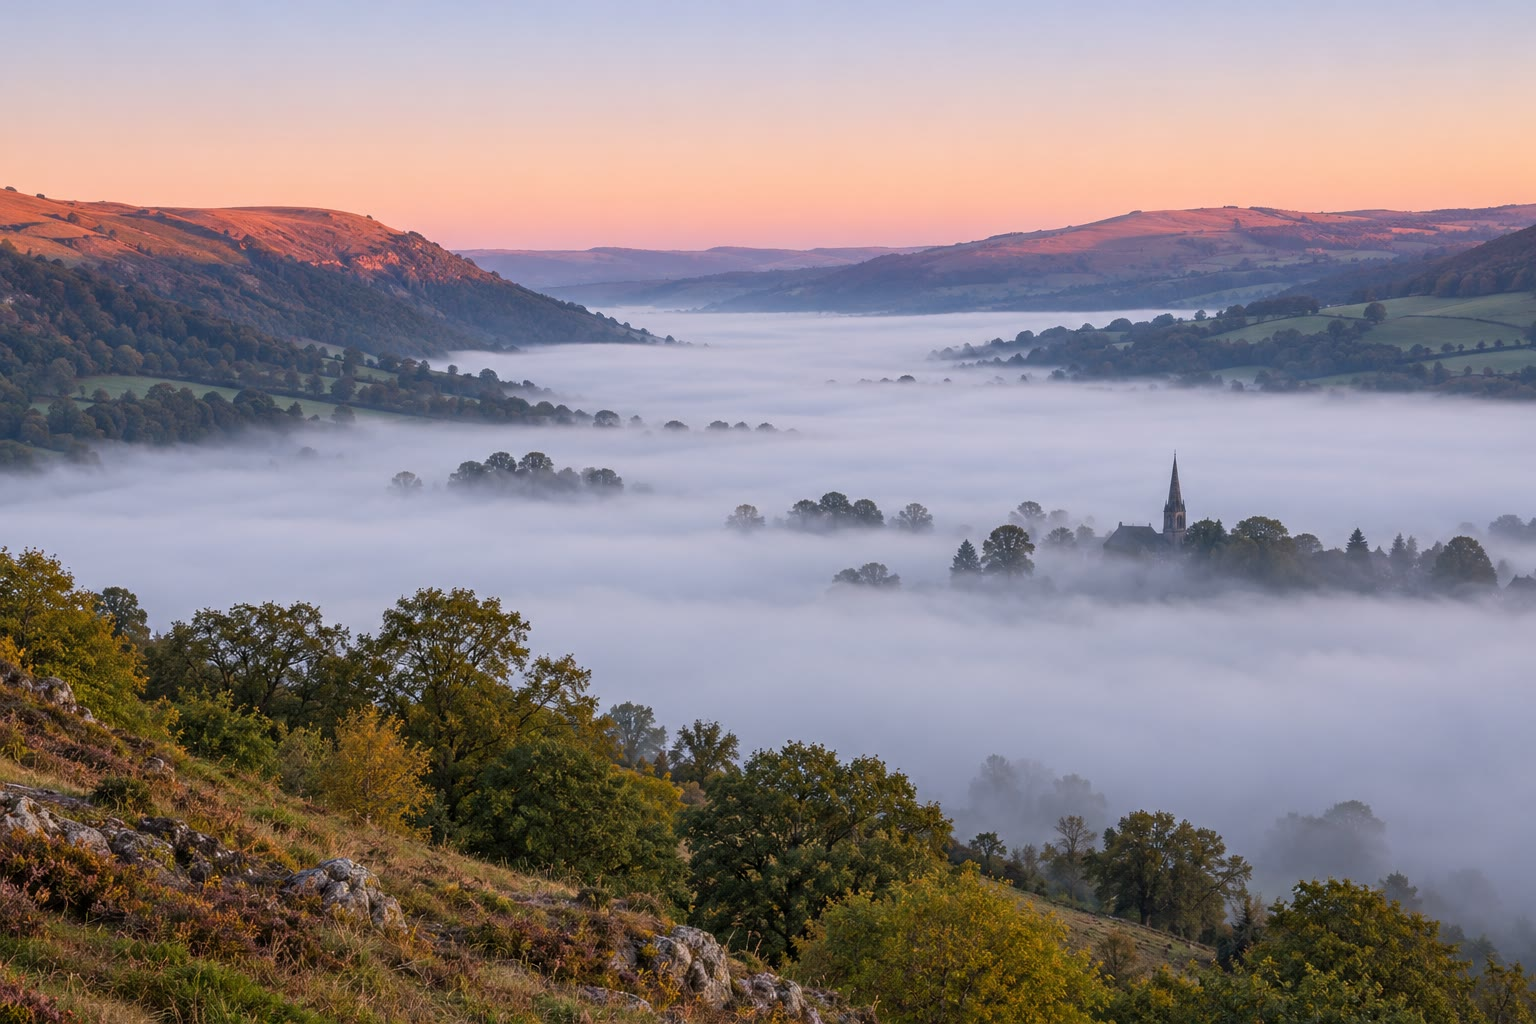
\includegraphics[width=0.75\linewidth]{images/book2/ai/g10-valley-fog.jpg}

{\small Du brouillard remplit une vallée à l'aube. Pendant la nuit claire,
le sol s'est refroidi, l'air froid s'est écoulé au fond de la vallée, et
là il s'est refroidi sous son \omterm{def:g10:why-clouds-form:dew-point}{point de rosée}.}
\end{omfigure}

\section{L'air qui monte se refroidit}

La plupart des nuages ne se forment pas parce que l'air touche quelque chose
de froid. Ils se forment parce que l'air monte. La pression diminue avec
l'altitude~; une parcelle d'air qui s'élève se dilate en repoussant l'air
environnant, et l'énergie de ce travail est prise à la parcelle elle-même.

\begin{definition}[Refroidissement adiabatique~; gradient adiabatique sec]\label{def:g10:why-clouds-form:adiabatic}
Le \emph{refroidissement adiabatique}\index{refroidissement adiabatique}
est le refroidissement d'une parcelle d'air qui se dilate sans échanger de
chaleur avec son environnement. Le taux auquel de l'air non \omterm{def:g10:why-clouds-form:humidity}{saturé} qui
monte se refroidit ainsi est le \emph{gradient adiabatique
sec}\index{gradient adiabatique sec}, proche de \qty{9.8}{\degreeCelsius}
par kilomètre d'ascension~; l'air qui descend se réchauffe au même taux.
\end{definition}

\begin{proposition}[Le gradient adiabatique sec]\label{prop:g10:why-clouds-form:dry-rate}
Le \omterm{def:g10:why-clouds-form:adiabatic}{gradient adiabatique sec} vaut $g/c_p$, où $g = \qty{9.81}{m/s^2}$ et $c_p
\approx \qty{1005}{J.kg^{-1}.K^{-1}}$ est l'énergie qui réchauffe un
kilogramme d'air d'un degré à pression constante~: $9.81/1005 \approx
\qty{0.0098}{\degreeCelsius/m}$, soit \qty{9.8}{\degreeCelsius/km}.
(Admis~: la démonstration relève des livres de physique.)
\end{proposition}
% ledger: const:gn, const:R, earth:Mmol (c_p of dry air computed as (7/2)R/M in figdata/grade-10/clouds.py)

Le \omterm{def:g10:why-clouds-form:dew-point}{point de rosée} de la parcelle diminue lui aussi quand elle monte, mais
lentement~: sa teneur en eau reste la même, tandis que la baisse de pression
rend la vapeur un peu plus facile à saturer. Le calcul, pour de l'air proche
du sol, donne environ \qty{1.8}{\degreeCelsius} par kilomètre. La
température de la parcelle se rapproche donc de son \omterm{def:g10:why-clouds-form:dew-point}{point de rosée}
d'environ $9.8 - 1.8 = \qty{8}{\degreeCelsius}$ par kilomètre d'ascension.
% ledger: iapws:vapour-pressure (dew-point rate computed in figdata/grade-10/clouds.py)

\begin{definition}[Niveau de condensation]\label{def:g10:why-clouds-form:condensation-level}
Le \emph{niveau de condensation}\index{niveau de condensation} d'une
parcelle d'air est l'altitude à laquelle, en montant, elle devient saturée.
L'eau se condense au-dessus~: le niveau de condensation est la base plate
des nuages que forme l'air ascendant.
\end{definition}

\begin{proposition}[Altitude du niveau de condensation]\label{prop:g10:why-clouds-form:lcl}
De l'air qui monte depuis le sol avec une température $T$ et un \omterm{def:g10:why-clouds-form:dew-point}{point de
rosée} $T_d$ (en \unit{\degreeCelsius}) devient \omterm{def:g10:why-clouds-form:humidity}{saturé} à environ
\[
  z = \frac{T - T_d}{8}\ \text{km} = \qty{125}{m} \times (T - T_d).
\]
\end{proposition}

\begin{proof}
À une altitude $z$ (en km), la température de la parcelle vaut
$T - 9.8\,z$ et son \omterm{def:g10:why-clouds-form:dew-point}{point de rosée} $T_d - 1.8\,z$. Elle est saturée quand
ils sont égaux~: $T - 9.8\,z = T_d - 1.8\,z$, donc $8\,z = T - T_d$ et
$z = (T - T_d)/8$ km. Un huitième de kilomètre vaut \qty{125}{m}.
\end{proof}

\begin{example}[Un cumulus d'après-midi]\label{ex:g10:why-clouds-form:base}
% ledger: iapws:vapour-pressure (exact ascent computed in figdata/grade-10/clouds.py: 1.51 km)
L'après-midi de l'\cref{ex:g10:why-clouds-form:morning}, l'air au sol est à
\qty{28}{\degreeCelsius} avec un \omterm{def:g10:why-clouds-form:dew-point}{point de rosée} de
\qty{16}{\degreeCelsius}. Les bulles qui montent deviennent \omterm{def:g10:why-clouds-form:humidity}{saturées} à
$125 \times 12 = \qty{1500}{m}$~: les cumulus ont leur base plate vers
\qty{1.5}{km} d'altitude. Le matin, à \qty{20}{\degreeCelsius}, le même air
se serait condensé dès $125 \times 4 = \qty{500}{m}$~: la base des nuages
s'élève au cours de la journée, à mesure que le sol se réchauffe.
\end{example}

\section{Air stable et air instable}

Qu'une parcelle qui monte continue de monter dépend de l'air qui l'entoure.
Une parcelle plus chaude que son environnement est plus légère que l'air
qu'elle déplace et monte, comme une montgolfière~; une parcelle plus froide
que son environnement redescend.

\begin{definition}[Air stable~; air instable]\label{def:g10:why-clouds-form:stability}
L'air est \emph{stable}\index{air stable} lorsqu'une parcelle poussée vers
le haut devient plus froide que l'air qui l'entoure, et redescend donc à son
point de départ. Il est \emph{instable}\index{air instable} lorsque la
parcelle devient plus chaude que l'air qui l'entoure et continue de monter
d'elle-même.
\end{definition}

La parcelle qui monte se refroidit au \omterm{def:g10:why-clouds-form:adiabatic}{gradient adiabatique sec},
\qty{9.8}{\degreeCelsius} par kilomètre, tant qu'elle n'est pas saturée.
Une fois saturée, elle se refroidit plus lentement~: la condensation libère
de la \omterm{def:g10:earth-energy-budget:latent-heat}{chaleur latente} dans la parcelle. Le calcul donne environ
\qty{4.7}{\degreeCelsius} par kilomètre dans l'air chaud proche du sol,
environ \num{5.8} à \qty{0}{\degreeCelsius}, et davantage dans l'air froid
plus haut, où il reste peu d'eau à condenser~; c'est le gradient
adiabatique \omterm{def:g10:why-clouds-form:humidity}{saturé}. (Sa formule est établie dans les volumes
universitaires.)
% ledger: nist:water-latent, iapws:vapour-pressure (saturated rates computed in figdata/grade-10/clouds.py)

\begin{method}[Cet air est-il stable~?]\label{met:g10:why-clouds-form:stable}
\begin{enumerate}
  \item Déterminer à quel rythme la température de l'air environnant
        diminue avec l'altitude (le gradient thermique vertical, tiré d'un
        radiosondage).
  \item Le comparer au rythme auquel la parcelle se refroidit~: le
        gradient sec, environ \qty{9.8}{\degreeCelsius/km}, sous son \omterm{def:g10:why-clouds-form:condensation-level}{niveau
        de condensation}~; le gradient \omterm{def:g10:why-clouds-form:humidity}{saturé}, environ
        \qty{5}{\degreeCelsius/km}, au-dessus.
  \item Si l'environnement se refroidit plus lentement que la parcelle,
        celle-ci finit plus froide~: l'air est \omterm{def:g10:why-clouds-form:stability}{stable}. S'il se refroidit
        plus vite, la parcelle finit plus chaude~: l'air est \omterm{def:g10:why-clouds-form:stability}{instable}. Une
        couche où la température \emph{augmente} avec l'altitude est très
        \omterm{def:g10:why-clouds-form:stability}{stable}~: elle arrête l'air qui monte comme un couvercle.
\end{enumerate}
\end{method}

Avec le gradient moyen d'environ \qty{6.5}{\degreeCelsius/km}, l'air est
\omterm{def:g10:why-clouds-form:stability}{stable} tant qu'il n'est pas \omterm{def:g10:why-clouds-form:humidity}{saturé} (la parcelle se refroidit plus vite) et
\omterm{def:g10:why-clouds-form:stability}{instable} une fois \omterm{def:g10:why-clouds-form:humidity}{saturé} (la parcelle se refroidit plus lentement). On dit
d'un tel air qu'il est conditionnellement \omterm{def:g10:why-clouds-form:stability}{instable}~: il est \omterm{def:g10:why-clouds-form:stability}{stable} à moins
que quelque chose ne le soulève jusqu'à son \omterm{def:g10:why-clouds-form:condensation-level}{niveau de condensation}, et
alors le nuage grandit de lui-même.

\begin{omfigure}
\begin{tikzpicture}
\begin{axis}[omrecord, width=0.9\linewidth, height=7.6cm, xmin=-30, xmax=36,
  ymin=0, ymax=6, xlabel={température (\unit{\degreeCelsius})}, ylabel={altitude (km)},
  xtick={-30,-20,...,30}, ytick={0,1,...,6},
  legend style={at={(0.02,0.98)}, anchor=north west, font=\footnotesize, draw=black!30, fill=white},
  tick label style={font=\small}, label style={font=\small}]
\fill[omDef!10] (axis cs:-30,1.51) rectangle (axis cs:36,3.96);
\addplot[black!60, thick] table[x=T_C, y=z_km] {figdata/out/grade-10-clouds-envA.dat};
\addlegendentry{radiosondage A}
\addplot[omProp!90!black, thick, densely dotted] table[x=T_C, y=z_km] {figdata/out/grade-10-clouds-envB.dat};
\addlegendentry{radiosondage B}
\addplot[omThm!85!black, very thick] table[x=T_C, y=z_km] {figdata/out/grade-10-clouds-parcel.dat};
\addlegendentry{parcelle qui monte}
\addplot[omMeth!85!black, thick, dashed] table[x=Td_C, y=z_km] {figdata/out/grade-10-clouds-dew.dat};
\addlegendentry{son point de rosée}
\draw[black!50, dashed] (axis cs:-30,1.51) -- (axis cs:36,1.51);
\node[anchor=south west, font=\footnotesize] at (axis cs:-29.5,1.53) {niveau de condensation};
\node[anchor=north east, font=\footnotesize, omDef!80!black] at (axis cs:35.5,3.9) {nuage avec A};
\end{axis}
\end{tikzpicture}

{\small Une parcelle qui monte depuis le sol à \qty{28}{\degreeCelsius} avec
un \omterm{def:g10:why-clouds-form:dew-point}{point de rosée} de \qty{16}{\degreeCelsius} (calcul)~: elle se refroidit
au gradient sec jusqu'à ce que sa température rejoigne son \omterm{def:g10:why-clouds-form:dew-point}{point de rosée} à
\qty{1.5}{km}, puis au gradient \omterm{def:g10:why-clouds-form:humidity}{saturé}, plus lent. Deux radiosondages
inventés~: avec A, la parcelle est plus chaude que son environnement de
\qty{1.5}{km} jusqu'à la couche chaude vers \qty{4}{km}, et un cumulus
grandit entre les deux (zone ombrée)~; avec B, de l'air plus chaud
au-dessus du sol maintient partout la parcelle plus froide que son
environnement~: \omterm{def:g10:why-clouds-form:stability}{air stable}, pas de cumulus.}
\end{omfigure}
% ledger: iapws:vapour-pressure, nist:water-latent (parcel computed in figdata/grade-10/clouds.py; soundings invented)

Quand l'air est \omterm{def:g10:why-clouds-form:stability}{stable} et qu'il est malgré tout soulevé --- par une
montagne, ou le long d'un front ---, les nuages qui se forment s'étalent en
couches grises et plates~: les stratus. Quand il est \omterm{def:g10:why-clouds-form:stability}{instable}, les nuages
bourgeonnent vers le haut en amas~: les cumulus, et, quand l'instabilité
monte assez haut, les cumulonimbus des orages, dont le sommet s'étale en
enclume là où il rencontre l'air très \omterm{def:g10:why-clouds-form:stability}{stable} situé au-dessus de la couche
la plus basse de l'atmosphère.

\begin{omfigure}
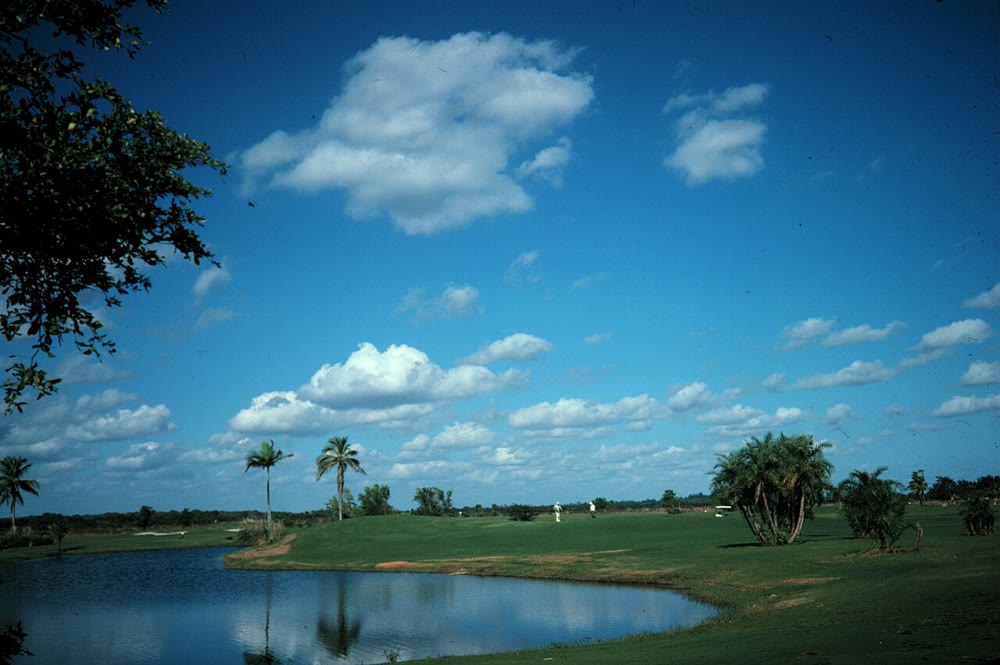
\includegraphics[height=4.5cm]{images/book2/g10-noaa-fair-weather-cumulus.jpg}\hspace{0.6em}%
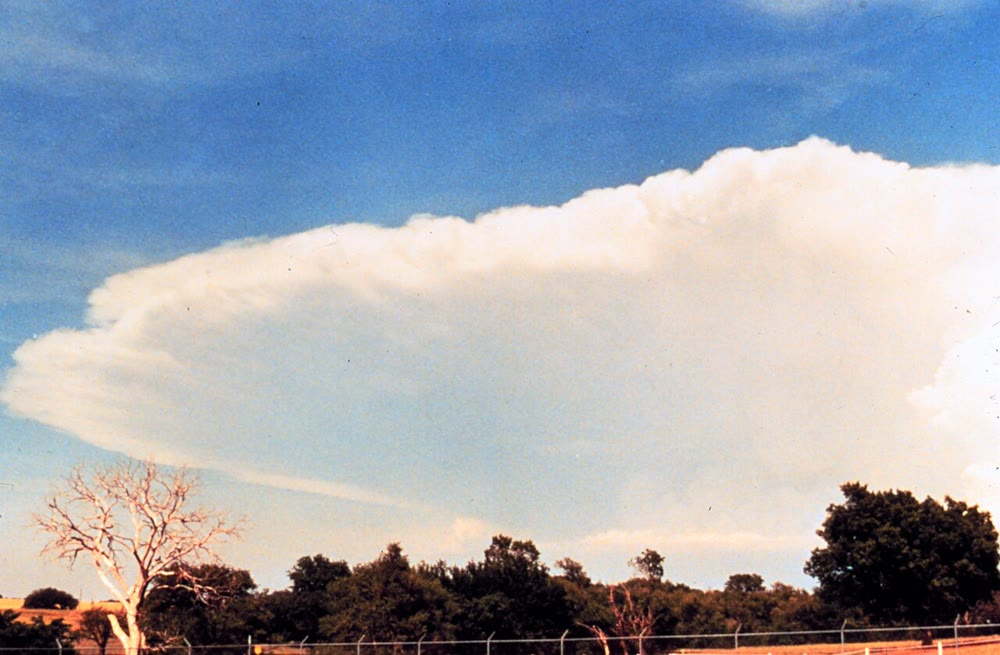
\includegraphics[height=4.5cm]{images/book2/g10-noaa-cumulonimbus-anvil.jpg}

{\small À gauche~: des cumulus de beau temps au-dessus de la Floride, avec
leur base plate au \omterm{def:g10:why-clouds-form:condensation-level}{niveau de condensation}. Photographie~: Ralph F. Kresge,
NOAA (domaine public). À droite~: l'enclume d'un cumulonimbus aux premiers
stades d'un orage. Photographie~: NOAA National Severe Storms Laboratory
(domaine public).}
\end{omfigure}

\section{Quatre façons de soulever l'air}

L'air monte pour quatre raisons.
\begin{itemize}
  \item \textbf{Le chauffage par le bas.} Par une journée ensoleillée, le
        sol réchauffe l'air qui le surmonte~; des bulles d'air chaud
        s'élèvent des zones les plus chaudes. Elles donnent les cumulus de
        l'après-midi.
  \item \textbf{Les montagnes.} Le vent qui souffle contre une chaîne de
        montagnes est forcé de monter le long de sa pente.
  \item \textbf{Les fronts.} Là où des masses d'air chaud et froid se
        rencontrent, l'air chaud, plus léger, monte par-dessus l'air froid,
        ou l'air froid s'insinue sous lui (livre~1, année~8).
  \item \textbf{La convergence.} Quand les vents confluent près du sol,
        l'air n'a d'autre issue que de monter, comme dans la ceinture d'air
        ascendant proche de l'équateur et au centre d'une dépression.
\end{itemize}

\begin{method}[Suivre une parcelle au-dessus d'une montagne]\label{met:g10:why-clouds-form:mountain}
\begin{enumerate}
  \item Trouver le \omterm{def:g10:why-clouds-form:condensation-level}{niveau de condensation} avec la règle des 125 mètres~;
        jusqu'à ce niveau, la parcelle se refroidit de
        \qty{9.8}{\degreeCelsius/km}.
  \item De là jusqu'à la crête, elle se refroidit au gradient \omterm{def:g10:why-clouds-form:humidity}{saturé}~;
        l'eau qui se condense tombe en pluie ou en neige sur le versant au
        vent.
  \item Au-delà de la crête, la parcelle descend, non saturée~: elle se
        réchauffe de \qty{9.8}{\degreeCelsius/km} jusqu'en bas.
\end{enumerate}
\end{method}

\begin{example}[Le vent chaud et sec du versant sous le vent]\label{ex:g10:why-clouds-form:lee}
% ledger: iapws:vapour-pressure, nist:water-latent (all values computed in figdata/grade-10/clouds.py)
De l'air au niveau de la mer à \qty{20}{\degreeCelsius}, avec un \omterm{def:g10:why-clouds-form:dew-point}{point de
rosée} de \qty{12}{\degreeCelsius}, est poussé par-dessus une crête haute de
\qty{2500}{m}. Il devient \omterm{def:g10:why-clouds-form:humidity}{saturé} à $125 \times 8 = \qty{1000}{m}$, vers
\qty{10}{\degreeCelsius}. De là jusqu'à la crête, il se refroidit au
gradient \omterm{def:g10:why-clouds-form:humidity}{saturé}, jusqu'à environ \qty{2}{\degreeCelsius}, et perd en pluie
environ un tiers de son eau (de \num{8.7} à \qty{6.0}{g/kg}). En
redescendant de l'autre côté, il se réchauffe au gradient sec sur
\qty{2.5}{km}~: il atteint la plaine à environ \qty{27}{\degreeCelsius},
sept degrés de plus qu'au départ, avec une \omterm{def:g10:why-clouds-form:humidity}{humidité relative} d'environ
\qty{27}{\percent}. De tels vents chauds et secs soufflent sous le vent de
nombreuses chaînes de montagnes.
\end{example}

\begin{omfigure}
\begin{tikzpicture}[font=\footnotesize, >={Stealth[length=2mm]}]
  \fill[omExo!30] (0,0) -- (3.5,0.3) -- (6,3.0) -- (8.5,0.3) -- (12,0) -- (12,-0.25) -- (0,-0.25) -- cycle;
  \draw[thick, black!70] (0,0) -- (3.5,0.3) -- (6,3.0) -- (8.5,0.3) -- (12,0);
  \draw[black!40, dashed] (0,1.2) -- (4.6,1.2);
  \node[anchor=south west, black!60, align=left] at (0.1,1.22) {niveau de\\condensation, \qty{1000}{m}};
  \foreach \x in {3.62,3.86,4.1} \draw[omDef!60] (\x,1.2) -- (\x-0.06,{0.3+(\x-0.06-3.5)*1.08+0.04});
  \pic[scale=1.1, transform shape] at (4.6,1.22) {puffycloud};
  \pic[scale=0.9, transform shape] at (5.0,2.2) {puffycloud};
  \draw[->, thick, omDef!80!black] (0.2,0.25) -- (2.8,0.5) .. controls (3.6,0.75) .. (4.4,1.7) -- (5.4,2.9) .. controls (5.8,3.4) and (6.2,3.4) .. (6.6,2.9) -- (7.6,1.7) .. controls (8.4,0.75) .. (9.2,0.5) -- (11.8,0.25);
  \node[anchor=east, align=right] at (3.4,2.15) {\qty{10}{\degreeCelsius}, saturé};
  \node[anchor=south, align=center] at (6.0,3.45) {crête \qty{2500}{m}~: \qty{2}{\degreeCelsius}};
  \node[anchor=west, align=left] at (7.75,2.1) {descend et se réchauffe\\de \qty{9.8}{\degreeCelsius/km}};
  \node[anchor=north, align=center] at (1.0,-0.3) {\qty{20}{\degreeCelsius}\\point de rosée \qty{12}{\degreeCelsius}};
  \node[anchor=north, align=center] at (11.0,-0.3) {\qty{27}{\degreeCelsius}\\point de rosée \qty{6}{\degreeCelsius}};
  \node[anchor=north, black!60] at (4.0,-0.3) {au vent~: pluie};
  \node[anchor=north, black!60] at (8.2,-0.3) {sous le vent~: sec};
\end{tikzpicture}

{\small Une parcelle d'air qui franchit une crête montagneuse (températures
calculées~; échelle verticale exagérée). Elle se refroidit au gradient sec
jusqu'à son \omterm{def:g10:why-clouds-form:condensation-level}{niveau de condensation}, au gradient \omterm{def:g10:why-clouds-form:humidity}{saturé}, plus lent,
au-dessus, en perdant de l'eau sous forme de pluie, et se réchauffe au
gradient sec pendant toute la descente du versant sous le vent.}
\end{omfigure}

\section{Des gouttelettes à la pluie et à la neige}

La vapeur d'eau ne se condense pas facilement dans un air parfaitement
propre. Les gouttelettes se forment sur des grains de matière.

\begin{definition}[Noyau de condensation]\label{def:g10:why-clouds-form:nucleus}
Un \emph{noyau de condensation}\index{noyau de condensation} est une
minuscule particule en suspension dans l'air --- un grain de sel marin, de
poussière, de fumée ou de suie --- sur laquelle la vapeur d'eau se condense
pour former une gouttelette de nuage.
\end{definition}

Un noyau typique mesure environ \qty{0.0002}{mm}, une gouttelette de nuage
environ \qty{0.02}{mm}, une goutte de bruine \qty{0.5}{mm} et une goutte de
pluie environ \qty{2}{mm}. Une goutte de pluie est cent fois plus large
qu'une gouttelette de nuage, donc son volume est $100^3$ fois plus grand~:
un million de gouttelettes de nuage font une goutte de pluie. Les
gouttelettes de nuage sont si petites que le moindre courant ascendant les
maintient en l'air~; pour qu'il pleuve, les gouttelettes doivent devenir
cent fois plus larges.
% ledger: jpl:drop-sizes

\begin{omfigure}
\begin{tikzpicture}
\begin{axis}[width=0.9\linewidth, height=3.4cm, xmode=log, xmin=1e-4, xmax=10,
  ymin=0, ymax=1, axis y line=none, axis x line*=bottom,
  xlabel={diamètre (mm), échelle logarithmique}, tick label style={font=\small},
  label style={font=\small}, clip=false]
\addplot[only marks, mark=*, omDef!85!black, mark size=2.5pt] coordinates {(0.0002,0.3) (0.02,0.3) (0.5,0.3) (2,0.3)};
\node[anchor=south, font=\footnotesize, align=center] at (axis cs:0.0002,0.42) {noyau de\\condensation};
\node[anchor=south, font=\footnotesize, align=center] at (axis cs:0.02,0.42) {gouttelette\\de nuage};
\node[anchor=south, font=\footnotesize, align=center] at (axis cs:0.5,0.42) {bruine};
\node[anchor=south, font=\footnotesize, align=center] at (axis cs:2,0.42) {goutte\\de pluie};
\end{axis}
\end{tikzpicture}

{\small Tailles typiques, sur une échelle où chaque pas vaut dix fois le
précédent~: chaque objet est environ cent fois plus large que le précédent,
sauf la bruine. Données~: NASA Jet Propulsion Laboratory.}
\end{omfigure}

Deux processus les font grossir.

\begin{definition}[Processus de la pluie chaude~; processus des cristaux de glace]\label{def:g10:why-clouds-form:rain-processes}
Dans le \emph{processus de la pluie chaude}\index{processus de la pluie chaude},
les plus grosses gouttelettes d'un nuage tombent plus vite que les petites,
les heurtent et fusionnent avec elles, grossissant au cours de leur chute.
Dans le \emph{processus des cristaux de
glace}\index{processus des cristaux de glace}, dans la partie d'un nuage
plus froide que \qty{0}{\degreeCelsius} où se mêlent des cristaux de glace
et des gouttelettes surfondues (liquides en dessous de
\qty{0}{\degreeCelsius}), les cristaux grossissent en captant la vapeur
qu'évaporent les gouttelettes~; ils tombent en flocons de neige, et fondent
en gouttes de pluie si l'air au-dessous est chaud.
\end{definition}

Le \omterm{def:g10:why-clouds-form:rain-processes}{processus des cristaux de glace} fonctionne parce que la teneur à
\omterm{def:g10:why-clouds-form:humidity}{saturation} est plus faible au-dessus de la glace qu'au-dessus de l'eau
liquide à la même température~: à \qty{-10}{\degreeCelsius}, la pression de
vapeur saturante vaut \qty{287}{Pa} au-dessus de l'eau et \qty{260}{Pa}
au-dessus de la glace. L'air \omterm{def:g10:why-clouds-form:humidity}{saturé} pour les gouttelettes contient
\qty{10}{\percent} de vapeur de plus que la glace ne peut en supporter~: la
vapeur se condense sur les cristaux, et les gouttelettes s'évaporent pour la
remplacer.
% ledger: iapws:vapour-pressure, iapws:melt-subl (computed in figdata/grade-10/clouds.py)

\begin{remark}[La chaleur latente nourrit l'orage]\label{rem:g10:why-clouds-form:latent}
Chaque kilogramme d'eau qui se condense dans un nuage cède à l'air environ
\qty{2.5}{MJ}, la \omterm{def:g10:earth-energy-budget:latent-heat}{chaleur latente} prise à la mer ou au sol lors de son
évaporation (\cref{ch:g10:earth-energy-budget}). C'est cette chaleur qui
rend le gradient \omterm{def:g10:why-clouds-form:humidity}{saturé} plus lent que le gradient sec et qui fait monter un
cumulonimbus~; le \cref{ch:g10:storms-and-cyclones} la suit jusque dans les
plus grandes tempêtes.
\end{remark}
% ledger: nist:water-latent

\section{Exercices}

Pour ces exercices, on utilisera les teneurs à \omterm{def:g10:why-clouds-form:humidity}{saturation} (en \unit{g/kg},
à la pression du niveau de la mer) du tableau ci-dessous, le gradient sec
\qty{9.8}{\degreeCelsius/km}, une baisse du \omterm{def:g10:why-clouds-form:dew-point}{point de rosée} de
\qty{1.8}{\degreeCelsius/km} et un gradient \omterm{def:g10:why-clouds-form:humidity}{saturé} de
\qty{5}{\degreeCelsius/km}.
% ledger: iapws:vapour-pressure (table from figdata/out/grade-10-clouds-sat.dat, rounded)

\begin{center}
\small
\begin{tabular}{l*{11}{c}}
\hline
température (\unit{\degreeCelsius}) & 0 & 4 & 8 & 10 & 12 & 14 & 16 & 20 & 24 & 28 & 30 \\
teneur à \omterm{def:g10:why-clouds-form:humidity}{saturation} (\unit{g/kg}) & 3.8 & 5.0 & 6.7 & 7.6 & 8.7 & 10.0 & 11.4 & 14.7 & 18.9 & 24.1 & 27.2 \\
\hline
\end{tabular}
\end{center}

\begin{exercise}[$\star$]\label{exo:g10:why-clouds-form:1}
Définir l'\omterm{def:g10:why-clouds-form:humidity}{humidité relative} et le \omterm{def:g10:why-clouds-form:dew-point}{point de rosée} de l'air.
\end{exercise}

\begin{exercise}[$\star$]\label{exo:g10:why-clouds-form:2}
À partir du tableau, donner la teneur à \omterm{def:g10:why-clouds-form:humidity}{saturation} à \num{0}, \num{10},
\num{20} et \qty{30}{\degreeCelsius}. Par quel facteur, à peu près,
est-elle multipliée pour chaque réchauffement de \qty{10}{\degreeCelsius}~?
\end{exercise}

\begin{exercise}[$\star$]\label{exo:g10:why-clouds-form:3}
De l'air à \qty{24}{\degreeCelsius} contient \qty{10.0}{g/kg} de vapeur
d'eau. Trouver son \omterm{def:g10:why-clouds-form:humidity}{humidité relative} et son \omterm{def:g10:why-clouds-form:dew-point}{point de rosée}.
\end{exercise}

\begin{exercise}[$\star$]\label{exo:g10:why-clouds-form:4}
Expliquer pourquoi un verre d'eau glacée «~transpire~» en été, et pourquoi
il ne le fait pas à l'intérieur par une journée d'hiver très sèche.
\end{exercise}

\begin{exercise}[$\star$]\label{exo:g10:why-clouds-form:5}
Nommer les quatre façons dont l'air est amené à monter, avec un exemple pour
chacune.
\end{exercise}

\begin{exercise}[$\star\star$]\label{exo:g10:why-clouds-form:6}
À l'aide de la \cref{prop:g10:why-clouds-form:lcl}, trouver l'altitude de
la base des nuages pour de l'air à \qty{30}{\degreeCelsius} avec un \omterm{def:g10:why-clouds-form:dew-point}{point de
rosée} de \qty{18}{\degreeCelsius}, et pour de l'air à
\qty{22}{\degreeCelsius} avec un \omterm{def:g10:why-clouds-form:dew-point}{point de rosée} de
\qty{20}{\degreeCelsius}. Quelle journée risque d'être grise, avec des
nuages bas~?
\end{exercise}

\begin{exercise}[$\star\star$]\label{exo:g10:why-clouds-form:7}
Une parcelle d'air non \omterm{def:g10:why-clouds-form:humidity}{saturé} quitte le sol à \qty{18}{\degreeCelsius}.
Quelle est sa température à \qty{1}{km} et à \qty{2}{km} d'altitude, si
elle reste non saturée~? En redescendant depuis \qty{2}{km}, à quelle
température atteint-elle le sol~?
\end{exercise}

\begin{exercise}[$\star\star$]\label{exo:g10:why-clouds-form:8}
Un radiosondage montre une température qui diminue de
\qty{4}{\degreeCelsius} par km. L'air est-il \omterm{def:g10:why-clouds-form:stability}{stable} pour une parcelle non
saturée~? Pour une parcelle saturée~? Par un après-midi chaud, la
température diminue de \qty{12}{\degreeCelsius} dans le premier kilomètre
au-dessus du sol~: que deviennent les bulles d'air chaud~?
\end{exercise}

\begin{exercise}[$\star\star$]\label{exo:g10:why-clouds-form:9}
De l'air \omterm{def:g10:why-clouds-form:humidity}{saturé} à \qty{20}{\degreeCelsius} est refroidi jusqu'à
\qty{10}{\degreeCelsius}. Combien de grammes d'eau se condensent par
kilogramme d'air~? Où va la \omterm{def:g10:earth-energy-budget:latent-heat}{chaleur latente} libérée~?
\end{exercise}

\begin{exercise}[$\star\star$]\label{exo:g10:why-clouds-form:10}
Combien de gouttelettes de nuage de \qty{0.02}{mm} de diamètre forment une
goutte de bruine de \qty{0.5}{mm} de diamètre~? Une goutte de pluie de
\qty{2}{mm} de diamètre~?
\end{exercise}

\begin{exercise}[$\star\star$]\label{exo:g10:why-clouds-form:11}
Expliquer, étape par étape, pourquoi le brouillard se forme dans les vallées
plutôt que sur les sommets des collines à l'aube, après une nuit claire et
calme.
\end{exercise}

\begin{exercise}[$\star\star\star$]\label{exo:g10:why-clouds-form:12}
Le gradient sec vaut $a$ et le \omterm{def:g10:why-clouds-form:dew-point}{point de rosée} diminue au taux $b$ (tous deux
en \unit{\degreeCelsius/km}). Montrer que le \omterm{def:g10:why-clouds-form:condensation-level}{niveau de condensation} est à
$z = (T - T_d)/(a - b)$. Au-dessus d'un haut plateau, le \omterm{def:g10:why-clouds-form:dew-point}{point de rosée}
diminue de \qty{1.7}{\degreeCelsius/km}~: que devient la règle
«~\qty{125}{m} par degré~»~?
\end{exercise}

\begin{exercise}[$\star\star\star$]\label{exo:g10:why-clouds-form:13}
De l'air au niveau de la mer à \qty{15}{\degreeCelsius}, avec un \omterm{def:g10:why-clouds-form:dew-point}{point de
rosée} de \qty{11}{\degreeCelsius}, franchit une crête haute de
\qty{2000}{m}. En suivant la \cref{met:g10:why-clouds-form:mountain},
trouver le \omterm{def:g10:why-clouds-form:condensation-level}{niveau de condensation}, la température à ce niveau, la
température à la crête, et la température à laquelle l'air atteint la
plaine de l'autre côté.
\end{exercise}

\begin{exercise}[$\star\star\star$]\label{exo:g10:why-clouds-form:14}
À \qty{-20}{\degreeCelsius}, la pression de vapeur saturante vaut
\qty{126}{Pa} au-dessus de l'eau et \qty{103}{Pa} au-dessus de la glace. De
quel pourcentage l'air \omterm{def:g10:why-clouds-form:humidity}{saturé} pour les gouttelettes est-il sursaturé pour
la glace~? Comparer à \qty{-10}{\degreeCelsius}, et dire dans quelle partie
d'un nuage le \omterm{def:g10:why-clouds-form:rain-processes}{processus des cristaux de glace} fonctionne le mieux.
\end{exercise}

\begin{exercise}[$\star\star\star$]\label{exo:g10:why-clouds-form:15}
L'air environnant se refroidit de \qty{6.5}{\degreeCelsius/km}. Une
parcelle part à la même température que son environnement et monte de
\qty{1}{km}. Calculer l'écart entre sa température et celle de
l'environnement si elle n'est pas saturée, puis si elle est saturée.
Expliquer l'expression «~conditionnellement \omterm{def:g10:why-clouds-form:stability}{instable}~».
\end{exercise}

\section{Problème~: un après-midi d'été sur la plaine}

\begin{problem}[{Problème du week-end --- de l'humidité du matin à la base
des nuages de l'après-midi}]
\label{pb:g10:why-clouds-form:1}
% ledger: iapws:vapour-pressure, nist:water-latent (all results computed in figdata/grade-10/clouds.py or from the rounded data below; the sounding is sounding A, invented)
Au-dessus d'une vaste plaine, par une journée d'été, l'air proche du sol
contient \qty{11.4}{g/kg} de vapeur d'eau toute la journée. Il est à
\qty{20}{\degreeCelsius} le matin et à \qty{28}{\degreeCelsius}
l'après-midi. Un radiosondage (un exemple inventé) donne la température de
l'air au-dessus~:

\begin{center}
\small
\begin{tabular}{l*{8}{c}}
\hline
altitude (km) & 0 & 0.5 & 1.0 & 1.5 & 2.5 & 3.5 & 3.6 & 4.0 \\
température (\unit{\degreeCelsius}) & 28.0 & 23.1 & 18.2 & 13.4 & 6.9 & 0.4 & $-0.3$ & 1.2 \\
\hline
\end{tabular}
\end{center}

\noindent On utilisera le tableau des teneurs à \omterm{def:g10:why-clouds-form:humidity}{saturation} et les gradients
donnés avant les exercices.

\medskip
\noindent\textbf{Partie I --- L'humidité.}
\begin{enumerate}
  \item Donner la teneur à \omterm{def:g10:why-clouds-form:humidity}{saturation} à \qty{20}{\degreeCelsius}.
  \item Calculer l'\omterm{def:g10:why-clouds-form:humidity}{humidité relative} du matin.
  \item Trouver le \omterm{def:g10:why-clouds-form:dew-point}{point de rosée} de l'air.
  \item Calculer l'\omterm{def:g10:why-clouds-form:humidity}{humidité relative} de l'après-midi.
  \item L'air est-il devenu plus sec l'après-midi~? Expliquer.
\end{enumerate}

\medskip
\noindent\textbf{Partie II --- La nuit et la rosée.}
\begin{enumerate}[resume]
  \item Pendant la nuit, l'air proche du sol se refroidit. À quelle
        température la rosée commence-t-elle à se former~?
  \item Si l'air se refroidit jusqu'à \qty{12}{\degreeCelsius}, combien de
        grammes d'eau par kilogramme d'air se sont condensés~?
  \item Pourquoi la rosée se forme-t-elle sur l'herbe et sur les toits des
        voitures avant de se former dans l'air~?
\end{enumerate}

\medskip
\noindent\textbf{Partie III --- Le radiosondage.}
\begin{enumerate}[resume]
  \item Calculer le rythme auquel la température diminue entre \num{0} et
        \qty{1.5}{km}. Le comparer au gradient sec.
  \item Le calculer entre \num{1.5} et \qty{3.5}{km}.
  \item L'air situé entre \num{1.5} et \qty{3.5}{km} est-il \omterm{def:g10:why-clouds-form:stability}{stable} pour une
        parcelle non saturée~? Pour une parcelle saturée~?
  \item Que se passe-t-il entre \num{3.6} et \qty{4.0}{km}~? Quel effet
        cela a-t-il sur un nuage qui monte~?
\end{enumerate}

\medskip
\noindent\textbf{Partie IV --- La base des nuages.}
\begin{enumerate}[resume]
  \item Calculer l'écart entre la température de l'air et son \omterm{def:g10:why-clouds-form:dew-point}{point de
        rosée} au sol l'après-midi.
  \item Calculer la température et le \omterm{def:g10:why-clouds-form:dew-point}{point de rosée} d'une bulle de cet
        air après une ascension de \qty{1}{km}, toujours non saturée.
  \item De combien l'écart entre les deux s'est-il réduit~? À quel rythme
        se réduit-il~?
  \item Montrer que ce rythme donne la règle «~\qty{125}{m} par degré~».
  \item Quelle aurait été la base des nuages le matin~?
  \item Expliquer pourquoi la base des cumulus s'élève au cours de la
        journée.
  \item Écrire l'équation qui exprime que la température de la bulle est
        égale à son \omterm{def:g10:why-clouds-form:dew-point}{point de rosée} à l'altitude $z$ (en km).
  \item La résoudre~: à quelle altitude se trouve la base des cumulus de
        l'après-midi~?
\end{enumerate}
\end{problem}
